% options:
% thesis=B bachelor's thesis
% thesis=M master's thesis
% czech thesis in Czech language
% english thesis in English language
% hidelinks remove colour boxes around hyperlinks


% arara: xelatex: { shell: yes }
% arara: makeglossaries	
% arara: biber
% arara: xelatex: { shell: yes }
% arara: xelatex: { shell: yes }
\documentclass[thesis=B,czech,hidelinks]{../template/FITthesisXE}

\usepackage{ graphicx }		% graphics files inclusion
\usepackage{ dirtree } 		% directory tree visualisation
\usepackage{ longtable } 	% tables which Pandoc use
\usepackage{ lscape }		% to be able to rotate stuff
\usepackage{ metalogo }		% for \XeLaTeX
\usepackage{ multicol }		% for multiple columns
\usepackage{ booktabs }		% for prettier tables
\usepackage{ rotating }		% for rotating pictures

\bibliography{sources.bib}

% make list of acronyms
\makeglossaries
\newacronym{BI-DBS}{BI-DBS}{Databázové systémy}
\newacronym{BI-SP1}{BI-SP1}{Softwarový týmový projekt 1}
\newacronym{BI-SP2}{BI-SP2}{Softwarový týmový projekt 2}
\newacronym{DBS}{DBS}{Databázové systémy}
\newacronym{FIT}{FIT}{Fakulta informačních technologií}
\newacronym{KOS}{KOS}{Komponenta studium}
\newacronym{LS}{LS}{letní semestr}
\newacronym{PMI}{PMI}{Project Management Institute}
\newacronym{RA}{RA}{Relational algebra / Relační algebra}
\newacronym{SQL}{SQL}{Structured query language}
\newacronym{XP}{XP}{Extrémní programování}
\newacronym{ZS}{ZS}{zimní semestr}
\newacronym{ČVUT}{ČVUT}{České vysoké učení technické}
\newglossaryentry{gCI}{
	name=Continuous integration,
	description={
		Systém automatického sestavování a testování změn zdrojového kódu.
		}
	}
\newglossaryentry{gCommit_message}{
	name=commit message,
	description={
		Krátká zpráva připojená ke \emph{commitu}, která shrnuje, co commit řeší.
		}
	}
\newglossaryentry{gCommit}{
	name=commit,
	description={
		Aplikování či přijmutí nových změn zdrojového kódu. V tomto textu používáno především v souvislosti s \emph{Gitem}.
		}
	}
\newglossaryentry{gConverse}{
	name=konverzní poměr,
	description={
		Pravděpodobnost, že se z návštěvníka stane zákazník.
		}
	}
\newglossaryentry{gCron}{
	name=cron,
	description={
		Služba operačního systému, která umožňuje v určitý čas nebo v určitých intervalech spouštět nějaký příkaz nebo skript.
		}
	}
\newglossaryentry{gDML}{
	name=Data manipulation language,
	description={
		Soubor klíčových slov se stanovenou syntaxí, podobný programovacímu jazyku, určený pro manipulaci s daty uloženými v databázi. Nejznámější DML je součástí SQL.
		}
	}
\newglossaryentry{gFeature}{
	name=Feature,
	description={
		Vlastnost, funkce, rys.
		}
	}
\newglossaryentry{gFramework}{
	name=Framework,
	description={
		Softwarová struktura, která slouží jako podpora pro pohodlnější programování. Může obsahovat podpůrné funkce, knihovny či nástroje pro efektivnější, bezpečnější a pohodlnější vývoj softwaru.
		}
	}
\newglossaryentry{gGitlab}{
	name=Gitlab,
	description={
		Nástavba nad Gitem ulehčující používání repozitáře ve webovém rozhraní.
		}
	}
\newglossaryentry{gGit}{
	name=Git,
	description={
		Distribuovaný systém pro správu verzí vhodný především pro soubory s textovým obsahem.
		}
	}
\newglossaryentry{gGrido}{
	name=Grido,
	description={
		PHP komponenta umožňující jednoduchý výpis dat do tabulky, jejich řazení, filtrování, stránkování a hromadné akce.
		}
	}
\newglossaryentry{gMerge}{
	name=merge,
	description={
		Sloučení dvou vývojových větví v \emph{Gitu}.
		}
	}
\newglossaryentry{gMvp}{
	name=Model-View-Presenter,
	description={
		\emph{Návrhový vzor} softwaru, který klade důraz na oddělení jednotlivých vrstev aplikace. Využívá jej například Nette Framework.
		}
	}
\newglossaryentry{gNette}{
	name=Nette,
	description={
		Webový framework pro PHP.
		}
	}
\newglossaryentry{gPull}{
	name=pull,
	description={
		Stažení nových změn větve ze sdíleného repozitáře do lokální složky.
		}
	}
\newglossaryentry{gPush}{
	name=push,
	description={
		Odeslání \emph{commitu} do sdíleného repozitáře, například Gitlabu.
		}
	}
\newglossaryentry{gSQLite}{
	name=SQLite,
	description={
		Jednoduchý databázový stroj, který uchovává celou databázi pouze v jednom souboru.
		}
	}
\newglossaryentry{gSlack}{
	name=Slack,
	description={
		Komunikační nástroj pro týmy.
		}
	}

\glsaddall

% % % % % % % % % % % % % % % % % % % % % % % % % % % % % % 

\acknowledgements{TODO poděkování}
\abstractCS{Práce se zaměřuje na efektivní řízení softwarového projektu, jehož cílem je vyvinout podpůrnou webovou aplikaci pro výuku předmětu BI-DBS na FIT ČVUT. Práce popisuje problémy s vedením vícečlenných týmů, zabývá se problematikou nasazování a udržitelnosti běhu výsledného softwaru a jeho průběžného vývoje. Cílem práce bylo navrhnout a začít používat postupy a nástroje, díky kterým se efektivně skloubí běžící systém a jeho průběžný vývoj za minimálního výskytu chyb. Jako metodika vývoje byla zvolena kombinace Extrémního programování a Feature-driven development, průběh práce je sledován v Redmine. Zdrojový kód aplikace je verzován a testován na Gitlabu. Poslední kapitola také obsahuje praktické ukázky konfigurace některých služeb potřebných pro běh samotné aplikace. Z práce lze vycházet při řízení jiných projektů obdobných rozměrů či pokračování v řízení stejného projektu.}
\abstractEN{This thesis focuses on effective software project management, which aims to develop a supporting application for teaching BI-DBS subject at FIT CTU. Thesis describes issues with leading a teams consisting of multiple people, deals with deployment, maintenance of deployed software and the development itself. The goal is to propose and start using procedures and tools, which will effectively combine a running system with its active development, while suppressing most of the bugs. The chosen software development methodology combines Extreme programming and Feature-driven development, the course of work is tracked in Redmine. Source code of the app is versioned and tested using Gitlab. The last chapter also includes samples of configuration for some services required to run the application. This work can be used as a base point for other projects with similar sizes or to continue in the process of managing the same project.}
\title {Řízení projektu a infrastruktury portálu pro podporu výuky předmětu BI-DBS}
\authorGN {Oldřich}
\authorFN {Malec}
\authorWithDegrees {Oldřich Malec}
\author {Oldřich Malec}
\supervisor {Ing. Jiří Hunka}
\keywordsCS {TODO}
\keywordsEN {TODO}
\department {Katedra softwarového inženýrství}
\placeForDeclarationOfAuthenticity {V~Praze}
\declarationOfAuthenticityOption {4}
\website {https://gitlab.fit.cvut.cz/malecold/bc-thesis}
\assignment {../pdf/zadani.pdf}


\begin{document}

%\input{hyphenation.tex}

\begin{introduction} \label{introduction}
Téma \emph{projektového řízení} je potřeba řešit u každého alespoň středně velkého projektu. Portál pro podporu výuky předmětu BI-DBS se již do takových rozměrů také dostal, především ve chvíli kdy je v jednu chvíli potřeba udržovat běh nasazené aplikace, opravovat chyby, které objevují koncoví uživatelé a řídit další vývoj nových funkcí. Kromě řízení projektu také práce obsahuje téma \emph{infrastruktury} vývoje softwaru, která zajišťuje efektivnější vývoj, komunikaci a plánování. Má působnost při řízení tohoto projektu a jeho infrastruktury by měla přispět k vyšší kvalitě používání zmíněné aplikace. Z výstupu by tedy měli těžit všichni studenti a vyučující předmětu BI-DBS.\\
Má motivace k řešení tohoto tématu vznikla ve chvíli, kdy jsem se v předmětu BI-SP2 stal vedoucím jednoho z týmů, které aplikaci vyvýjely pod vedením Jiřího Hunky. Viděl jsem, že mé programátorské schopnosti nedosahují takových úrovní jako některých ostatních studentů, kteří například naprogramovali celou kostru nového systému, zato jsem však měl cit pro procesy v projektovém řízení, svědomitost při záznamech stráveného času nebo zájem o nastavování postupů vývoje a konfigurace nových podpůrných služeb, potřebných pro běh i vývoj aplikace.\\
V práci nejprve seznámím čtenáře s předmětem BI-DBS, pro který je portál vyvíjen a přiblížím podobu řízení projektu, jak probíhalo před započetím mé práce. Následně se zabývám analýzou metodik vývoje softwaru, ze kterých tvořím závěry pro jejich využití při vývoji DBS portálu. Třetí kapitola obsahuje jak teorii, tak praxi při řízení lidských zdrojů, což je jedním z mých hlavních zaměření při práci na projektu. Čtvrtá a poslední kapitola popisuje veškeré podpůrné nástroje, ať už se jedná o konfigurace serveru nebo služby používané realizačním týmem, k jejichž nastavení nebo definici použivání jsem jistou měrou přispěl.\\
Práce by se dala zařadit k ostatním bakalářským a diplomovým pracem, které vznikly pro účely DBS projektu. Jejich autoři, chronologicky seřazeni podle termínu dokončení práce, jsou: Jan Sýkora, Martin Kubiš, Filip Glazar, Petr Pejša, Jiří Slavotínek, Tomáš Fedor, Pavel Kovář a Milan Vlasák.

TODO nějaká vlna
\end{introduction}

\chapter{Co je to DBS portál} \label{DBSportal}

Tato práce se zabývá především vývojem a správou portálu pro předmět BI-DBS na FIT ČVUT. Ještě než se tedy ponoříme do jednotlivých součástí vývoje tohoto portálu, chtěl bych čtenáře seznámit s předmětem samotným.

\section{Historie výuky BI-DBS}

Předmět Databázové systémy je vyučován na katedře softwarového inženýrství a v současném studijním programu se s ním setkají studenti bakalářského programu Informatika ve svém druhém semestru. Výuka si klade za cíl přiblížit studentům problematiku ukládání dat, a to především pomocí relačních databází. Důraz je kladen na jazyky RA a SQL. Forma výuky předmětu pochází již z dob výuky na FEL ČVUT a používala se již déle než 10 let.

\paragraph{Semestrální práce}
Každý student si v rámci své semestrální práce vytvoří vlastní databázi, kterou naplní testovacími daty a následně vymýšlí dotazy. Typická semestrální práce obsahuje ve své finální podobě alespoň 25 dotazů do a pokrývá všechny standardní klauzule DML, jednak z jazyku \emph{relační algerby} a také z SQL. DML v SQL vypadá následovně:
\begin{itemize}
	\item \code{SELECT ... FROM ... WHERE ... ;}
	\item \code{INSERT INTO ... VALUES ... ;}
	\item \code{UPDATE ... SET ... WHERE ... ;}
	\item \code{DELETE FROM ... WHERE ... ;}
\end{itemize}
Semestrální práce se vypracovávala ve formátu XML, který byl následně pro přehlednější reprezentaci převeden do HTML pomocí XSLT. Zejména studenti si často na nutnost vyplňování XML šablony stěžovali.

\paragraph{Testy v semestru a zkouška}
Kromě semestrálních prací popsaných výše jsou také součástí hodnocení studentů průběžné testy v semestru a závěrečná zkouška. Testy v semestru se týkají především praktické části - tedy používání RA a SQL či modelování schémat databáze - které by student měl mít osvojené ze své semestrální práce. Závěrečná zkouška poté kromě praktických částí může obsahovat i teoretické otázky které byly probírány na přednášce.

\section{Vznik DBS portálu} \label{DBSportal:creation}
Obě výše popsané součásti výuku jsou poměrně náročné na korekturu vyučujícím. Typicky nebylo možné zajistit, aby vyučující zkontroloval každý jednotlivý dotaz, který student vytvořil ve své semestrální práci. Oprava testů, které se psaly na papír poté trvala zbytečně dlouho a prakticky nebylo možné ji automatizovat. Z tohoto důvodu přišel v roce 2013 Jiří Hunka - jeden z vyučujících předmětu BI-DBS - s nápadem, že se realizuje portál zaměřený na podporu výuky Databázových systémů, který bude umožňovat jak efektivnější korekturu studentských semestrálních prací, tak rychlejší opravu testů a zkoušek.

\paragraph{Řešitelský tým}
Vývoj portálu takových rozměrů však nebylo možné financovat běžně dostupnými prostředky, kterými fakulta disponuje. Z toho důvodu bylo rozhodnuto, že bude portál vyvíjen s rámci předmětů BI-SP1 a BI-SP2. Jedná se o předměty vyučované také v oboru Softwarové inženýrství, které si studenti typicky zapisují ve svém 4., respektive 5. semestru studia. Cílem předmětů je vytvořit 3-5 členné týmy, které budou pracovat na softwarovém projektu, počínaje návrhem, analýzou požadavků atp. a konče hotovým softwarem. Bylo tak vypsáno zadání na realizaci DBS portálu, do kterého se přihlásilo 13 studentů.
Tento způsob získávání pracovní síly pro další vývoj portálu je používán dodnes. Jelikož SP1 a navazující SP2 má celkové trvání jeden akademický rok, jsou každý rok nabíráni noví studenti. Toto přináší jak obtíže s řízením projektu, tak příležitosti pro jeho změny. Řízení DBS projektu se věnuje kapitola \ref{DBSmanagement}.

\paragraph{Nasazení portálu}
Portál byl poprvé nasazen do výuky v LS 2016, kdy byl využíván pouze na cvičeních, která vedl Jiří Hunka a ve zkouškovém období byl otestován také na jednom termínu závěrečné zkoušky.
V ZS 2016 portál používali všichni studenti, kteří měli předmět BI-DBS zapsaný, protože jich v tomto semestru bylo pouze 36. Jednalo se tak o ideální testovací vzorek pro příští semestr. Následující semestr - LS 2017 - již byl portál využíván všemi cvičícími a počet studentů se pohyboval kolem 550. Detailům ohledně nasazování portálu se věnuje kapitola \ref{infrastructure}.

\section{Historie řízení vývoje portálu} \label{intro:management}

Já sám jsem se s portálem seznámil poprvé v letním semestru 2015 v rámci předmětu BI-SP1. V té době byla aplikace nasazena na testovací doméně, ale nebyla ještě používána \uv{veřejností}.\\
Další vývoj probíhal pomocí dvou řešitelských týmů po 4 členech, které navázaly na předchozí týmy. Projektové řízení bylo v té době - především z kapacitních důvodů - na velmi slabé úrovni: V týmech byli stanoveni vedoucí, kteří měli za práci týmu zodpovídat, ve skutečnosti však spíše pracoval každý sám za sebe. Hotová práce se poté prezentovala jednou týdně na schůzce s Jiřím Hunkou. Jeden z týmů měl navíc k dispozici ještě Jana Sýkoru, který zastával roli vedoucího týmu. Honza v té době pracoval na své bakalářské práci na téma \emph{Podpora automatizované kontroly semestrální práce z předmětu Databázové systémy} a týmům zadával úkoly pro realizaci jeho návrhů UI a funkcionality a výstup poté i kontroloval.\\
Po dokončení předmětů BI-SP1 a následně BI-SP2 jsem u projektu zůstal a začal jsem se naplno věnovat jeho projektovému řízení, správě infrastruktury a opravě kritických chyb. V současnosti vedu již druhý běh studentů BI-SP1 a mezitím vznikly i čtyři další bakalářské a jedna diplomová práce související s portálem.

\chapter{Metodiky vývoje softwaru} \label{methods}

V této kapitole čtenáře seznámím s jednotlivými metodikami vývoje softwaru a zaměříme se také na možnosti jejich použití při vývoji DBS portálu, který byl popisován v kapitole \ref{DBSportal}.	

\paragraph{Proč používat metodiku vývoje softwaru}
Ještě než začneme s představením jednotlivých metodik, měli bychom si říci, proč bychom vlastně měli nějakou metodiku vývoje používat.\\
Při práci na \emph{malém} softwaru, který píše pouze jedna osoba, je opravdu mnohdy zbytečené starat se o \emph{nějakou} vývojovou metodiku. Jakmile však chceme spojit práci více lidí, požadujeme aby výsledný produkt byl hotový do určitého termínu, splňoval všechny předem stanovené požadavky a byl udržovatelný i po jeho nasazení, začínáme mít potřebu zavádět určitá pravidla či předpisy, které nám pomohou všechny požadavky naplnit. Právě v tuto chvíli vstupují do hry \emph{metodiky vývoje softwaru}, které právě tento \uv{balík} pravidel předepisují a vedení projektu poté stačí zvolit nejvhodnější metodiku či jejich kombinaci pro daný projekt.

\section{Tradiční metodiky} \label{methods:traditional}

\subsection{Vodopádový model} \label{methods:waterfall}

Jak zmiňuje Kadlec \cite{kadlec}, nejedná se přímo o metodiku, ale pouze o životní cyklus. Je charakteristický tím, že všechny fáze vývoje jsou prováděny postupně za sebou a není možné se vracet. Případné změny je možné zpracovat až v rámci údržby, která vývoj vždy vrátí do jedné z předchozích etap a následně musí proběhnout i etapy následující.\\
Seznam vývojových fází:
\begin{itemize}
	\item Definice problému,
	\item Specifikace požadavků,
	\item Návrh,
	\item Implementace,
	\item Integrace, testování,
	\item Údržba.
\end{itemize}

\paragraph{Použití v DBS projektu}
Tento model je obecně pro dnešní vývoj softwaru nevhodný, jelikož software je typicky potřeba dodat nejprve se základní funkcionalitou a poté iterativně přidávat další funkce: přesně tak je vyvíjen i DBS portál.

%%%%%%%%%%%%%%%%%%%%%%%%%%%%%%
%%%%%%%%%%%%%%%%%%%%%%%%%%%%%%
%%%%%%%%%%%%%%%%%%%%%%%%%%%%%%

\subsection{Spirálový model} \label{methods:spiral}

Vzniku Spirálového modelu dala za vznik především kritika Vodopádového modelu. Hlavní novinkou zde byl \emph{iterativní přístup} a opakovaná \emph{analýza rizik}. V tomto modelu se stále opakují fáze \emph{Stanovení cílů}, \emph{Analýza rizik}, \emph{Vývoj a testování} a \emph{Plánování}. Při každém průchodu těmito fázemi se provádí odlišná činnost než v předchozí iteraci (kromě analýzy rizik, ta je prováděna vždy stejně), například fáze vývoje v první iteraci pracuje pouze s koncepty, v příští iteraci specifikuje požadavky, v další navrhuje architekturu a teprve poté implementuje a testuje.
Stále se však jedná převážně o jednosměrnou cestu, která nejen na počátku ale i v průběhu obsahuje velké množství analýz a návrhů.

\paragraph{Použití v DBS projektu}
Tato metodika sice zavádí iterace, ale ty jsou pouze čtyři základní, předem definované. Jak bylo zmíněné výše u vopádového modelu (\ref{methods:waterfall}), DBS projekt potřebuje být vyvíjen pomocí skutečně iterativní metodiky, která bude v jednotlivých iteracích přidávat funkcionality.

Tradičních metodik existuje samozřejmě větší množství, pro potřeby této práce jich však nebudu více uvádět a přesuneme se k Agilním metodikám.

%%%%%%%%%%%%%%%%%%%%%%%%%%%%%%
%%%%%%%%%%%%%%%%%%%%%%%%%%%%%%
%%%%%%%%%%%%%%%%%%%%%%%%%%%%%%

\section{Agilní metodiky} \label{methods:agile}

Agilní metodiky řízení vznikly především z důvodu neustále se měnících požadavků na software a rychlejší reakci na požadované změny. Tradiční metodiky nebyly schopné reagovat na změny požadavků dostatečně rychle. Především když se začneme bavit o vývoji softwaru, kde se neustále mění dostupné technologie a požadavky na finální verzi, jsou tradiční metodiky zcela nevhodným modelem vývoje.

Rozdíl mezi tradiční a agilní metodikou lze popsat také jejich přístupem k \emph{Funkcionalitě}, \emph{Času} a \emph{Zdrojům} (Kadlec \cite{kadlec}). Zatímco u tradičních metodik je funkcionalita stanovena na začátku a musí být dosažena pomocí \emph{nějakého} času a \emph{nějakého} množství zdrojů, u agilních metodik je to přesně naopak. Typicky je stanoven termín a dostupné zdroje a funkcionalita \emph{nějaká} bude.

Připomeňme si také \emph{Manifesto for Agile Software Development} \cite{manifesto}, který vznikl v roce 2001:

\begin{quote}
Objevujeme lepší způsoby vývoje software tím,
že jej tvoříme a pomáháme při jeho tvorbě ostatním.
Při této práci jsme dospěli k těmto hodnotám:
\begin{itemize}
	\item \emph{Jednotlivci a interakce} před procesy a nástroji.
	\item \emph{Fungující software} před vyčerpávající dokumentací.
	\item \emph{Spolupráce se zákazníkem} před vyjednáváním o smlouvě.
	\item \emph{Reagování na změny} před dodržováním plánu.
\end{itemize}
Jakkoliv jsou body napravo hodnotné,
bodů nalevo si ceníme více.

\begin{multicols}{3}
Kent Beck\\
Mike Beedle\\
Arie van Bennekum\\
Alistair Cockburn\\
Ward Cunningham\\
Martin Fowler\\
James Grenning\\
Jim Highsmith\\
Andrew Hunt\\
Ron Jeffries\\
Jon Kern\\
Brian Marick\\
Robert C. Martin\\
Steve Mellor\\
Ken Schwaber\\
Jeff Sutherland\\
Dave Thomas\\
\end{multicols}

{\color{gray}
© 2001, výše zmínění autoři
Toto prohlášení může být volně kopírováno v jakékoli formě,
ale pouze v plném rozsahu včetně této poznámky.
}

\end{quote}

Je tedy zřejmé, že Agilní metodiky více pracují s vývojáři samotnými, a umožňuji i potlačení některých postupů pro dobro celku a dovolují "zanedbat" i náležitosti jako například dokumentaci. Následně se na některé agilní metodiky zaměříme více:

%%%%%%%%%%%%%%%%%%%%%%%%%%%%%%
%%%%%%%%%%%%%%%%%%%%%%%%%%%%%%
%%%%%%%%%%%%%%%%%%%%%%%%%%%%%%

\subsection{Extrémní programování} \label{methods:XP}

Na začátek je vhodné říci, že je rozdíl mezi \emph{extrémním vývojem softwaru} a \emph{extrémním projektovým řízením}. Zatímco projektové řízení se dá dělit na tradiční, agilní a extrémní (Wysocki, \cite{wysocki}), u vývoje softwaru se naopak dá říci, že XP položilo základ pro agilní metodiky a je tak jednou z nich.

XP rozvíjí standardní postupy, avšak posouvá je až do extrémů:
\begin{itemize}
	\item Vždy budeme pracovat na co nejjednodušší verzi, která splňuje požadavky.
	\item Pokud se osvědčuje \emph{revize kódu}, budeme neustále revidovat kód \ldots
	\item Pokud se odvědčil \emph{návrh}, budeme neustále navrhovat a vylepšovat specifikaci \ldots
	\item Pokud se osvědčilo \emph{testování}, budeme neustále testovat \ldots
	\item Narozdíl od tradičních metodik, které najednou dodají velký balík nových funkcionalit, bude XP dodávat i ty nejmenší funkční kousky. Toto vede na \emph{krátké iterace}.
\end{itemize}

Tyto postupy přivedené do extrémů jsou reprezentovány v \emph{12 základních postupech XP}, se kterými se seznámíme níže.\\
Ještě než se dostaneme k samotným postupům, potřebujeme se seznámit s pojmem \emph{karta zadání.}

\paragraph{Karty zadání a karty úkolů} \label{methods:XP:issues}
Karty zadání vznikají během plánování návrhu softwaru. Tohoto plánování se účastní všichni vývojáři, vedení a i zákazník. Typicky jedna karta popisuje jednu funkcionalitu či jeden požadavek. Kartě náleží vlastnosti jako \emph{datum vytvoření}, \emph{stav}, \emph{priorita}, \emph{odhad vyřešení} a také samozřejmě vlastní zadání úkolu a dodatečné poznámky. Když se poté na jedné kartě pracuje, je aktualizována průběžnými poznámkami, které popisují které části již byly splněny, co je potřeba udělat atp.\\
Kromě karet zadání existují v XP také \emph{karty úkolů}. Tyto vznikají nikoliv na začátku celého procesu vývoje, ale na začátku jednotlivé iterace.

\paragraph{12 základních postupů XP} \label{methods:XP:12}
\begin{enumerate}
	\item \emph{Plánovací hra:} Probíhá jednak na začátku vývoje v rámci návrhu celé aplikace, tak na začátku jednotlivých iterací. Jejím výstupem jsou \emph{Karty zadání} a \emph{Karty úkolů}, popisované v předchozím odstavci.
	\item \emph{Malé verze:} Verze jsou dodávány neustále. I nejmenší změna funkcionality, která přináší užitek pro zákazníka je vydána jako nová verze.
	\item \emph{Metafora:} Celý systém je popisován jednoduchým příběhem, jak má ve výsledku fungovat. Tento příběh je sdílen jak vývojáři a managementem, tak zákazníkem a případně dalšími zainteresovanými osobami. Tato metafora u XP nahrazuje tradiční popis architektury.
	\item \emph{Jednoduchý návrh:} XP navrhuje vždy pouze to, co je přímo požadováno. Žádné přidáné vlastnosti nechce do návrhu zahrnovat, snaží se udělat minimum pro to, aby byly splněny požadavky.
	\item \emph{Testování:} Během vývoje jsou neustále psány i testy pro nově vznikající komponenty. Nikdy nesmí existovat jednotka, která nemá vlastní unit test. Testy dokonce píší i sami zákazníci, kteří tvoří testy funkcionality.
	\item \emph{Refaktorizace:} Refaktorizace je změna zdrojového kódu, která ovšem nemění jeho chování. Je prováděna z důvodu zvýšení čitelnosti kódu pro ostatní programátory či jeho zefektivnění. V XP by měl programátor vždy buď pouze implementovat novou funkčnost, nebo refaktorizovat stávající kód.
	\item \emph{Párové programování:} Zdrojový kód je vždy psán dvěma programátory u jednoho počítače. Zatímco jeden píše kód, druhý sleduje postup a přemýšlí nad dalšími souvislostmi: Je tato funkce napsána správně? Zapadá do celkového konceptu? Změní tato úprava chování jiného modulu? Je potřeba napsat nový test? \ldots
	\item \emph{Společné vlastnictví:} Zatímco některé jiné metodiky přiřazují jednotlivé třídy určitým programátorům, které za ně poté mají zodpovědnost, v XP je to právě naopak. Všichni mají zodpovědnost za celý kód a kdokoliv tak může měnit libovolnou součást systému.
	\item \emph{Nepřetržitá integrace:} Systém je sestaven a otestván vždy, jakmile je to možné, typicky tedy ihned po dokončení nové funkcionality.
	\item \emph{Čtyčicetihodinový pracovní týden:} XP klade důraz i na spokojenost lidských zdrojů. Snaží se tedy o nepřetěžování programátorů, jelikož při jejich únavě se razantně snižuje kvalita jejich výstupu.
	\item \emph{Zákazník na pracovišti:} Součastí týmu by měl být i sám zákazník, neboli expert na cílovou doménu. Jeho účelem je odpovídat na dotazy, tvořit testy či určovat priority.
	\item \emph{Standardy pro psaní zdrojového kódu:} Jelikož XP nedefinuje žádné standardní dokumenty, jsou veškeré informaci o projektu obsaženy ve zdojových kódech samotných. Proto je potřeba, aby byly rozumně strukturované, čitelné a pochopitelné.
\end{enumerate}

\paragraph{Použití v DBS projektu}
Některé z těchto postupů jsou jistým způsobem používány i při vývoji DBS portálu, více v sekci \ref{methods:dbs}.

%%%%%%%%%%%%%%%%%%%%%%%%%%%%%%
%%%%%%%%%%%%%%%%%%%%%%%%%%%%%%
%%%%%%%%%%%%%%%%%%%%%%%%%%%%%%

\subsection{Scrum} \label{methods:scrum}

Scrum je charakterizován především pojmy \emph{Sprint} a \emph{Scrum meeting}. První z nich má trvání většinou jeden měsíc a opakuje se několikrát. Jeho cílem je přinést do výsledného produktu nové funkcionality. Naopak Scrum meeting je \emph{každodenní} schůzka, na které se shrnou nově dokončené úkoly a stanoví se, na čem se bude dále pracovat. Schůzku vede tzv. \emph{Scrum master}. Typicky probíhá ve stoje a netrvá déle než 30 minut. Dalo by se říci, že tyto každodenní schůzky jsou stěžejní aktivitou metodiky Scrum. Od těchto schůzek se také odvíjí velikost týmu: Scrum preferuje malé týmy mezi třemi až šesti členy.

\paragraph{Použití v DBS projektu}
Pro potřeby DBS projektu je tedy Scrum také nevhodný, především jelikož předpokládá každodenní schůzky.

%%%%%%%%%%%%%%%%%%%%%%%%%%%%%%
%%%%%%%%%%%%%%%%%%%%%%%%%%%%%%
%%%%%%%%%%%%%%%%%%%%%%%%%%%%%%

\subsection{Feature driven development} \label{methods:fdd}

Jak název napovídá, FDD se soustředí především na \emph{featury}, neboli jednotlivé vlastnosti, funkce či rysy výsledného softwaru. Na počátku je vytvořen základní model softwaru, který je dále členěn na jednotlivé vlastnosti. Vývoj probíhá zpravidla v dvoutýdenních iteracích, jejichž výsledkem by měl vždy být fungující software, který je možné představit zákazníkovi.

Klíčový pojem \emph{feature (vlastnost)}  lze popsat jako samostatnou část systému, která splňuje následující parametry:
\begin{itemize}
	\item \emph{Měritelnost}: vlastnost je jasně uchopitelná komponenta systému, kterou lze porovnat s požadavkem zákazníka.
	\item \emph{Srozumitelnost}: programátor musí rozumět tomu, jak má vlastnost fungovat a co je jejím cílem.
	\item \emph{Realizovatelnost}: programátor musí vědět, zda je schopen vlastnost realizovat v odpovídajícím časovém úseky (typicky iterace 2 týdny). V opačném případě je většinou potřeba vlastnost rozdělit na více menších, a na těch pracovat samostatně.
\end{itemize}

V tuto chvíli by se mohlo zdát, že FDD vůbec nedisponuje \emph{návrhem a modelováním}. Ve skutečnosti je tomu právě naopak, společně s FDD je často zmiňován ještě \emph{model-driven approach}. Jelikož vlastnosti jsou klíčovou stavební jednotkou FDD, je potřeba je kvalitně navrhnout a namodelovat.

Posloupnost kroků při vývoji pomocí FDD zachycuje následující seznam:
\begin{enumerate}
	\item vytvoření celkového (globálního) modelu,
	\item vypracování podrobného seznamu vlastností,
	\item plánování podle vlastností,
	\item návrh podle vlastností,
	\item implementace.
\end{enumerate}
Dvě poslední se poté stále opakují, dokud existují další vlastnosti, které je potřeba pro softwaru přidávat.

Vzhledem k vývoji DBS portálu zde stojí za zmínku především fáze návrhu a implementace:

\paragraph{Návrh}
Vlastnosti se vždy týkají různých tříd, za které má zpravidla zodpovědnout určitá osoba, či dané třídě nejvíce rozumí určitý programátor. Ti jsou tedy rozděleni do týmů dle potřeby a sestavení týmů se tak pro každou iteraci obměňuje.\\
Tento nově sestavený tým má poté za úkol připravit návrh implementace vlasnosti, na jehož základě je poté naprogramována.

\paragraph{Implementace}
Týmy sestavené v předchozí fázi pracují na vlastní funkcionalitě nové vlastnosti. Společně s programovým kódem jsou tvořeny i testy, a to především \emph{unit testy}.\\
Jakmile je vlastnost dokončena, je vložena do sdíleného prostoru, u FDD nazývaného \emph{class repository}\\
Hlavní programátor poté dokončené vlastnosti integruje do předchozí verze hlavní aplikace.

Typicky na projektu pracuje několik týmů a hlavní progragramátor poté pouze volí nové vlastnosti k implementaci a integruje hotové vlastnosti do výsledné aplikace.

\paragraph{Použití v DBS projektu}
Výše popsaný průběh práce hrubě odpovídá i organizaci vývoje DBS projektu, které je popsáno v sekci \ref{methods:dbs}.

%%%%%%%%%%%%%%%%%%%%%%%%%%%%%%
%%%%%%%%%%%%%%%%%%%%%%%%%%%%%%
%%%%%%%%%%%%%%%%%%%%%%%%%%%%%%

\subsection{Test driven development} \label{methods:tdd}

Součástí každého vývojového procesu je bezesporu i testování výstupu. TDD této skutečnosti využívá a posouvá tvorbu testů ještě před samotný zdrojový kód aplikace. Při přidávání funkcionality do systému je tedy nejprve napsán test, který bude funkcionalitu testovat. Požadovaná funkcionalita je poté naprogramována přesně tak, aby procházela testy. Testy samozřejmě stále přibývají a tak je zapotřebí, aby nová funkcionalita prošla nejen novým testem napsaným přímo pro ni, ale také všemi ostatními.
Tento přístup vyžaduje jisté odhodlání programátora, jelikož vždy na první pohled vypadá jednodušeji pouze \emph{dopsat tu jednu řádku}. Při korektním postupu pomocí TDD je však i pro nejmenší změnu kódu vždy potřeba napsat test.

\paragraph{Použití v DBS projektu}
Jelikož TDD se svým konceptem \emph{test first, program later} vzdaluje od klasických vývojových metodik, není vhodné pro vývoj DBS portálu, kde se každý rok mění složení programátorů. DBS projekt samozřejmě využívá testy, viz kapitola \ref{version:gitlab:tests}, testuje se však vždy funkcionalita, která již existuje. Testy tedy především hlídají, zda změny v kódu nepoškodily jinou funkcionalitu, a testy pro nové funkce jsou dopsány až poté, co je funkční.



Na předchozích stránkách jsme si představili \emph{některé} vývojové metodiky. Především těch agilních však existuje nepřeberné množství, a jak říká například Kadlec \cite{kadlec} nebo Rasmusson \cite{rasmusson}, každý projekt je jedinečný a určitě není nejlepší možností striktně dodržovat jednu z vývojivých metodik. Klíčem je spíše skloubení dostupných metodik k vytvoření vlastní, pro daný projekt nejefektivnějšího přístupu k vývoji. Vedoucí týmu či projektový manažer by neměl \emph{slepě} následovat recept předložený například Extrémném programováním a zamítat jakékoliv jeho úpravy. Z toho důvodu i pro DBS projekt vznikla vlastní metodika, které se bude věnovat jak následující sekce, tak celá následující kapitola.

%%%%%%%%%%%%%%%%%%%%%%%%%%%%%%
%%%%%%%%%%%%%%%%%%%%%%%%%%%%%%
%%%%%%%%%%%%%%%%%%%%%%%%%%%%%%

\section{Zvolené řešení pro DBS projekt} \label{methods:dbs}

Jak bylo zmíněno v sekcích o \emph{\nameref{methods:XP}} a \emph{\nameref{methods:fdd}}, DBS projekt je vyvíjem pomocí metodiky na pomezí XP a FDD.

Na následujících řádcích budu pro potřeby této kapitoly popisovat i nástin \emph{infrastruktury}, která se v DBS projektu využívá. Tomuto tématu je však věnována také vlastní kapitola \ref{infrastructure}.

%%%%%%%%%%%%%%%%%%%%%%%%%%%%%%
%%%%%%%%%%%%%%%%%%%%%%%%%%%%%%
%%%%%%%%%%%%%%%%%%%%%%%%%%%%%%

\subsection{Inspirace v XP}

Jedním z požadavků vývoje pomocí \emph{Extrémního programování} je předpoklad, že budou dodržovány všechny jeho náležitosti. Jelikož jsme však na akademické půdě a vývojáři DBS projektu jsou především studenti předmětů BI-SP1, případně BI-SP2 (více v kapitole \nameref{DBSportal}), není možné abychom využívali například \emph{párové programování} či \emph{čtyřicetihodinový pracovní týden}, které XP \uv{předepisuje}.
Už minimálně z tohoto důvodu nemůže být XP použito ve svém plném obsahu. Důvodu je více, nyní se však pojďme zaměřit naopak na to, co vývoj DBS portálu z Extrémního programování \emph{využívá:}

\paragraph{Revize kódu}
XP mluví o neustálé revizi kódu. Jelikož studenti, kteří portál programují, jsou často nezkušení, je opravdu důležité jejich kód často revidovat, ideálně ihned po jejich \emph{commitu} do \emph{Gitu}. Revize provádí vedoucí týmu a také vedení projektu, zejména Pavel Kovář.

\paragraph{Krátké iterace, malé verze}
Jelikož DBS portál je \emph{webová aplikace}, je velmi jednoduché vydat novou verzi. Toho je také využíváno a nové veřejné verze jsou publikovány téměř každý týden. Kromě toho jsou publikovány i testovací verze, které je možné používat paralelně s produkční verzí a zde jsou změny nasazovány dle potřeby - někdy i vícekrát denně.

\paragraph{Karty zadání}
XP popisuje \emph{Karty úkolů} (\ref{methods:XP:issues}), které víceméně odpovídají úkolům, které jsou v DBS projektu zadávány v \emph{Redmine}. Odpovídají zejména pole jako \emph{datum}, \emph{stav}, \emph{priorita} či \emph{průběžné poznámky plnění}.

Obecně se ale dá říct, že takovouto funkci \emph{issue trackeru} musí určitý systém plnit prakticky v \emph{jakékoliv} vývojové metodice, mluvit o \emph{inspiraci z XP} tak u tohoto bodu nemá takový dopad.

\paragraph{Testování a nepřetržitá integrace}
V XP je \uv{předepsáno} neustále dopisovat testy pro nově vznikající komponenty. To probíhá i při vývoji DBS portálu, což je podpořeno i \emph{neustálou integrací}. Jakmile je dopsána nová funkčnost, tak při jejím \emph{push}i do \emph{Gitlab}u se automaticky spustí \gls{gCI}.

\paragraph{Zákazník na pracovišti}
Tato součást není při vývoji DBS portálu dodržována zcela, již z důvodu, že prakticky neexistuje sdílené pracoviště. Jednotliví členové pracují typicky odděleně, kdekoliv.
Zákazník ovšem \emph{je} součástí týmu. V případě DBS projektu se jedná o Jiřího Hunku, vedoucího této práce, který jakožto vyučující předmětu BI-DBS je zároveň jedním z hlavních uživatelů výsledné aplikace. Určuje tedy priority, testuje nové verze a hlásí chyby či požadavky.
\\
\\
\\
Vývoj DBS portálu tedy přebírá z Extrémního programování zhruba \emph{polovinu} jeho základních postupů (\ref{methods:XP:12}). Dále se pojďme zaměřit na to, co je přebráno z \nameref{methods:fdd}.

%%%%%%%%%%%%%%%%%%%%%%%%%%%%%%
%%%%%%%%%%%%%%%%%%%%%%%%%%%%%%
%%%%%%%%%%%%%%%%%%%%%%%%%%%%%%

\subsection{Inspirace v FDD}

I z \nameref{methods:fdd} jsou přebrány některé metodiky vývoje pro DBS projekt. Především rozdělení na jednotlivé \emph{featury} a role \emph{hlavního programátora}:

\paragraph{Featury} Ve FDD je vývoj hnán kupředu především seznamem vlastností, které má finální podoba mít. Toho využívá i DBS projekt, u kterého takový seznam existuje a z jedné strany se stále rozšiřuje novými požadavky, na straně druhé je zpracováván programátory. Jednotlivé vlastnosti jsou meřitelné, v případě jejich nesrozumitelnosti jsou programátorovi dopřesněny a jsou člěneny tak, aby byly realizovatelné do následující iterace (1-2 týdny).

\paragraph{Hlavní programátor}
Ve FDD dominuje role \emph{hlavního programátora}, který určuje priority jednotlivých vlastností připravených k implementaci a integruje jejich hotové řešení do výsledné aplikace. Tuto roli zastávám v DBS projektu já, jakožto \emph{projektový manažer}. Mým úkolem je mimo jiné zpracovávat požadavky a nahlášené chyby do jednotlivých zadání. Této činnosti se blíže věnují mnohé z následujících sekcí, jak z kapitoly \nameref{DBSmanagement}, tak \nameref{infrastructure}.

\chapter{Řízení lidských zdrojů} \label{DBSmanagement}

Řízení lidských zdrojů je jednou z neobtížnějších součástí projektového řízení, především proto, že se prolíná s dalšími odvětvími jako například \emph{psychologií} či \emph{sociologií}. Jelikož lidé jsou hnací silou projektu, mohou různé metody či samotná kvalita (ba dokonce absence!) řízení lidských zdrojů odrážet výsledný úspěch či neúspěch projektu. I v DBS projektu tedy vyvstala potřeba tuto pozici zaujmout a chopil jsem se jí já, jak již bylo popsáno v kapitole \ref{intro:me}.

\subsection{Role psychologie v řízení lidí}
Ještě než se ponoříme do samotných procesů popisujících řízení lidkých zdrojů, věnujme se chvíli právě oněm dalším odvětvím, které se s řízením lidí prolínají. Jak již bylo řečeno, jedná se především o \emph{psychologii}.

Lidé nejsou stroje, kterým poskytneme určitý vstup a podle jeho množství můžeme očekávat výstup. Je potřeba se zamýšlet nad dalšími okolnostmi, proč pro nás daný člověk pracuje, zda je spokojený, kdy odvádí nejlepší práci atp. Za veškerou lidskou činností stojí \emph{nějaká} motivace, cílem projektového manažera je poté najít, co motivuje právě jemu svěřené pracovníky.

\paragraph{\nameref{picture:maslow}}
\begin{figure}[h]
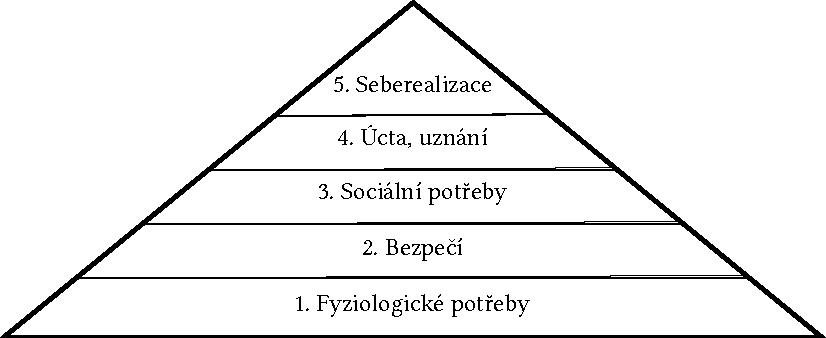
\includegraphics[width=\textwidth]{../pdf/maslow.pdf}
\caption{Maslowova pyramida potřeb} \label{picture:maslow}
\end{figure}

Ve standardních projektech, kde jsou vývojáři odměňováni finančně, se dá plat považovat za splnění základních fyziologických potřeb, protože je za něj možné nakoupit právě jídlo či pití. V DBS projektu jsou namísto finančně studenti hodnoceni známkou z předmětu, který je pro jejich studijní obor povinný. Jelikož však \emph{vystudování vysoké školy} obecně je spíše potřebou \emph{úcty, uznání} či \emph{seberealizace}, jedná se o vyšší patra pyramidy. Maslow tvrdí, že není možné uspokojovat vyšší patra pyramidy, pokud nejsou zajištěny ty nižší. Z toho důvodu může být obtížné motivovat k práci ty studenty, kteří nejprve potřebují vyřešit své zabezpečení (1. a 2. úroveň pyramidy), takoví studenti budou logicky dávat přednost před prací na projektu opravdové práci, za kterou dostanou peníze. Jakmile však má student zajíštěné tyto \uv{nižší potřeby}, dostávají se do popředí právě ty, které může DBS projekt nabídnout. Toto otevírá skvělé možnosti pro rozvoj jak samotných studentů, tak výsledného portálu. Jako příklad uvedu Pavla Kováře, který v tuto chvíli pracuje na bakalářské práci na téma \emph{Automatizované testování webového portálu dbs.fit.cvut.cz}. K projektu se dostal stejnou cestou jako já (viz kapitola \ref{intro:me}), ale o rok později. Po dokončení předmětu BI-SP2 se rozhodl u projektu zůstat a pokračovat v jeho vývoji. Jelikož již během vývoje v rámci SP týmů sám od sebe přicházel s inovacemi a kvalitními návrhy na zlepšení, jedná se dle mého názoru o jasný příklad naplňování nejvyšší potřeby, a to \emph{seberealizace}.\\
Právě seberealizace je jedna z potřeb, na kterou se snažím při řízení DBS projektu klást důraz. Studenti jsou hodnoceni jednak za práci, která je jim zadána, navíc ale dostávají příležitosti rozvíjet vlastní nápady a přínosy projektu a jsou za tyto přínosy také kladně hodnoceni. Více o hodnocení je popisováno v sekci \ref{ppl:ranking}.

TODO Schwalbe: 356+?

\subsection{Procesy řízení lidských zdrojů}

Jak popisuje Schwalbe \cite{schwalbe} ve své knize \emph{Řízení projektů v IT: kompletní průvodce}, při řízení lidských zdrojů se rozeznávají následující procesy:
\begin{itemize}
	\item Vytvoření plánu lidských zdrojů
	\item Zajištění projektového týmu
	\item Rozvoj projektového týmu
	\item Řízení projektového týmu
\end{itemize}
V následujících sekcích si jednotlivé procesy rozebereme pordobněji a zaměříme se i na jejich roli v DBS projektu.

%%%%%%%%%%%%%%%%%%%%%%%%%%%%%%
%%%%%%%%%%%%%%%%%%%%%%%%%%%%%%
%%%%%%%%%%%%%%%%%%%%%%%%%%%%%%

\section{Vytvoření plánu lidských zdrojů}

Cílem tohoto procesu je vytvořit plán, jaké \emph{typy} lidí potřebujem do projektu zapojit. Může se jednat například o \emph{profesionálního C++ programátora} či \emph{webdesignéra s citem pro UI a UX} atp. Typicky je vytvořena stromová struktura, kterou zastřešuje projektový manažer a dále se dělí například na jednotlivé části - programátoři, testeři, grafici, z nichž například programátoři mohou být dále rozděleni do týmů starajících se o jednotlivé komponenty systému, kde každý tým má ještě svého vedoucího. Takovému plánu se říká \emph{OBS} (Organization Breakdown Structure) a měla by být vytvořena na začátku projektu a podle ni následně zvoleni vedoucí daných oblastí.

\paragraph{Použití v DBS projektu}
V DBS projektu popisuje organizační členění obrázek \ref{picture:obs}.\\
\begin{figure}[h]
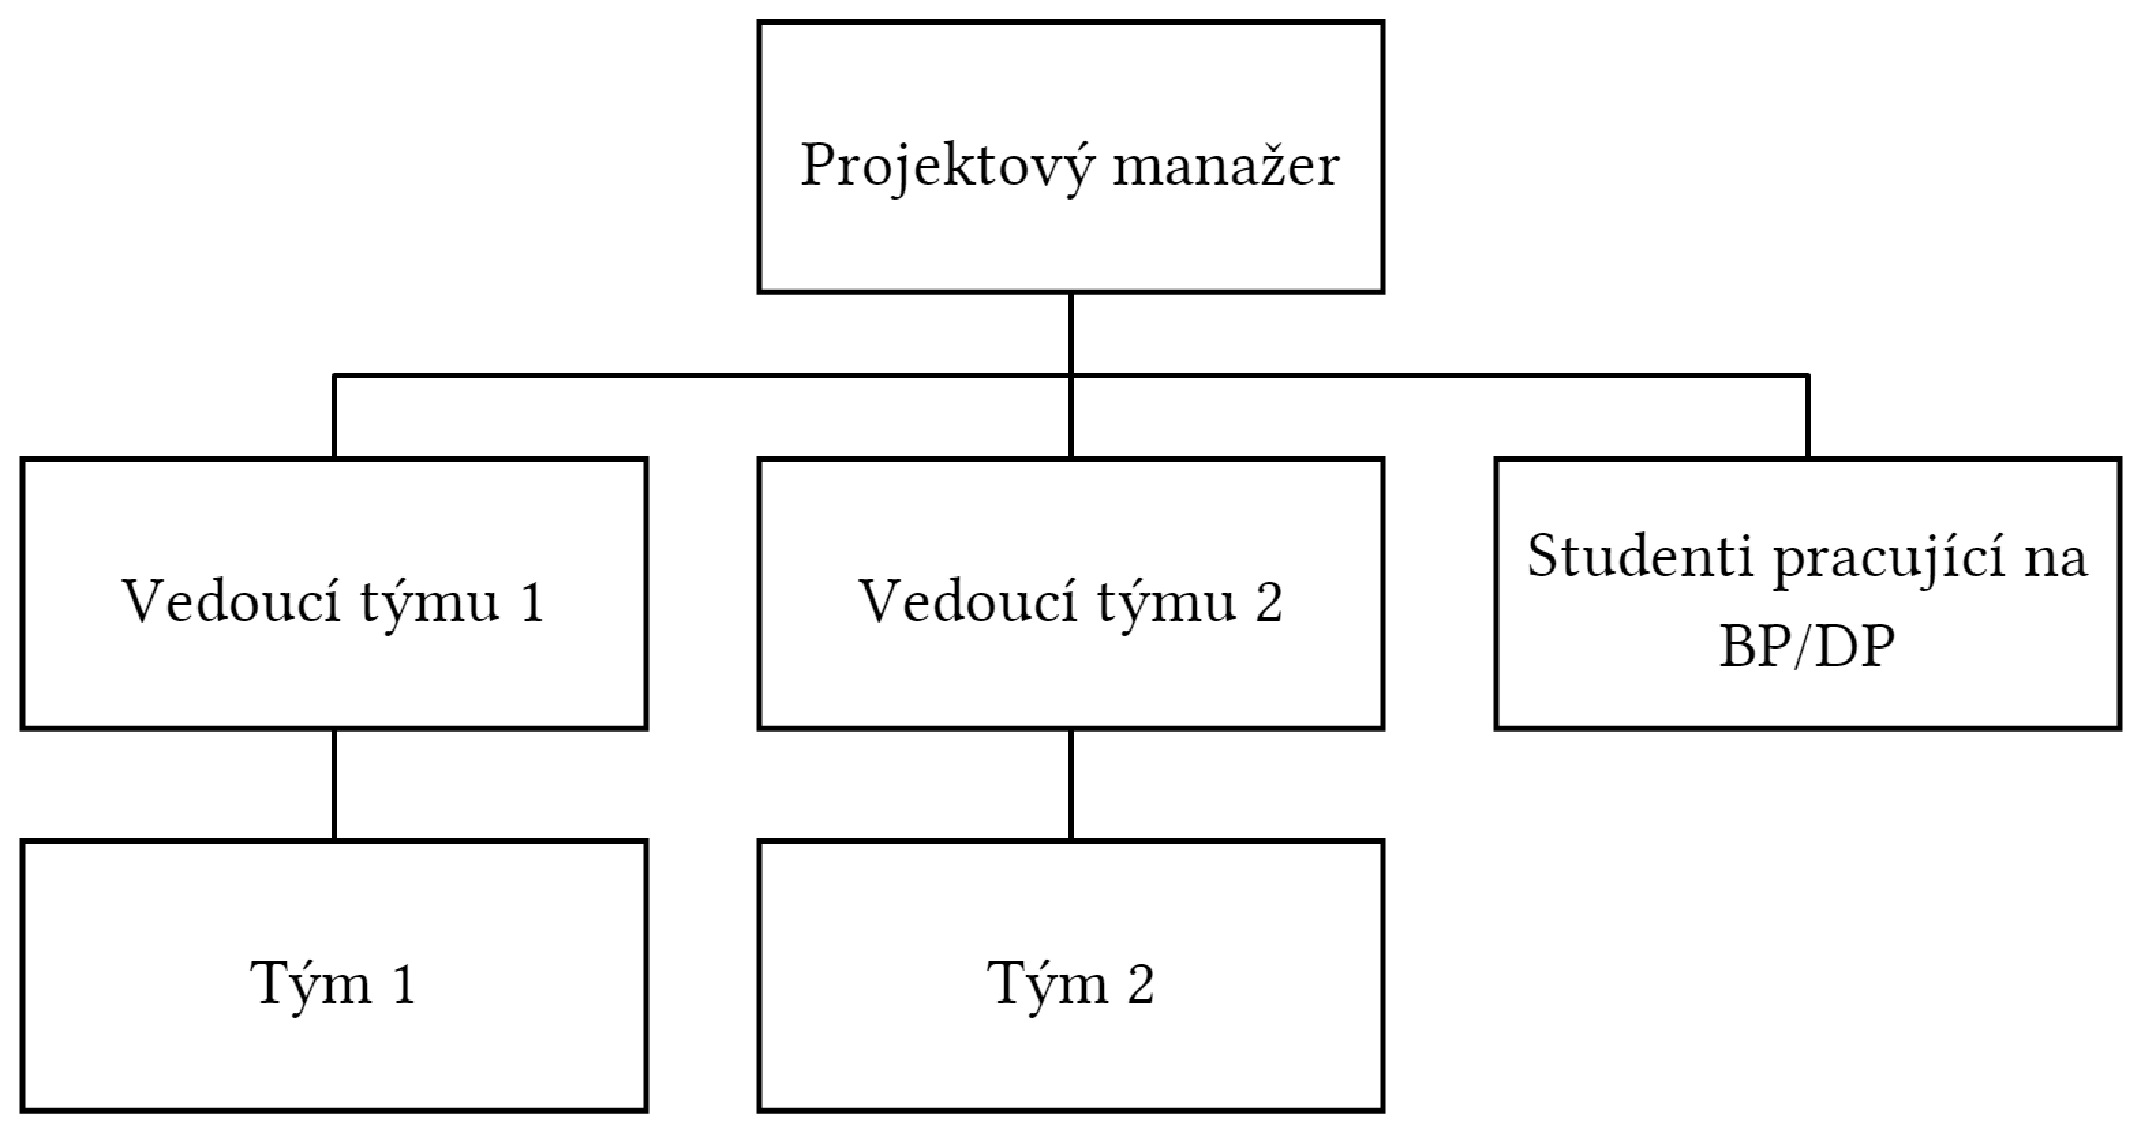
\includegraphics[width=\textwidth]{../pdf/dbs-obs.pdf}
\caption{Organization Breakdown Structure používaná v DBS projektu} \label{picture:obs}
\end{figure}
Je však nutné přiznat, že tato struktura v případě našeho projektu vznikla spíše \emph{na základě dostupných lidí}, než naopak, jak by to být mělo. Dělení na týmy fungovalo již od začátku, vedoucí týmu však často nezvládal dodržovat svou práci (více v úvodní kapitole \ref{intro:management}). Teprve po dalším zastřešení jejich zodpovědnosti \emph{projektovým manažerem} se stala pozice vedoucího týmu důležitější, a to především na úrovni komunikace manažera s týmem. Veškěré úkoly, kterou manažer do týmu zadává, prochází přes vedoucího týmu, který práci dále rozděluje, a po jejím dokončení opět kontroluje. Tento proces je znázorněn i na activity diagramu v příloze \ref{picture:activity}.

%%%%%%%%%%%%%%%%%%%%%%%%%%%%%%
%%%%%%%%%%%%%%%%%%%%%%%%%%%%%%
%%%%%%%%%%%%%%%%%%%%%%%%%%%%%%

\section{Zajištění projektového týmu}

Tento proces se primárně stará o \emph{příjem nových pracovníků}, \emph{řízení jejich vytížení} a \emph{vyrovnání}. První ze zmíněných je především v IT hodně diskutované téma, kdy najít člověka se správnou kvalifikací je často nadlidský úkol. Firmy se tak přetahují kdo nabídne zajímavější pracovní prostředí, lepší benefity či \emph{evergreen}: vyšší plat.\\
Když už je \emph{ten správný} zaměstnanec přijat, je potřeba řídit jeho \emph{vytížení} a případně jeho vznik \emph{vyrovnávat}: Jedná se o metodiky, kde je sledována práce přiřazená zaměstnanci a v případě, že je po něm požadování více, než je schopen zvládnout, je buďto přehodnocen harmonogram a úkoly s nižší prioritou jsou odloženy na později, nebo je k úkolu přiřazen další pracovník.\\
Plánování přiřazení práce je důležité především z důvodu předcházení výkyvů v množství přidělené práce, což vede na větší pohodlí zaměstnance a také snadnější řízení. 

\subsection{Použití v DBS projektu}
Jelikož u DBS projektu se pohybujeme na akademické půdě a nikoliv ve světě byznysu, je zde přístup k náboru nových pracovníků trochu odlišný. Noví pracovníci - studenti - jsou shánění jednak nárazově jednou ročně - při startu nového letního semestru, a také kontinuálně - jakožto zájemci o bakalářskou či diplomovou práci.\\
První ze zmíněného náboru vyžaduje vypsání tématu na stránku předmětu BI-SP1, kde se snažíme studenty nalákat právě k našemu projektu. Především v tomto roce (2017) se zvýšila zajímavost ostatních nabízených projektů (různé mobilní aplikace atp.), a tak se i zde začal projevovat podobný efekt jako u reálných firem, a to \emph{lov pracovníků}. Zároveň jsme však po nových studentech chtěli, aby měli buďto zkušenost s použitými technologiemi, nebo měli předpoklad k rychlému naučení těchto - pro někoho nových - technologií. Z toho důvodu jsme připravili \emph{vstupní kvíz} (viz níže podsekce \nameref{DBSmanagement:quiz}), který měl původně sloužit jako nutný požadavek pro vstup do týmů, z důvodu nízkého zájmu však byla poté jeho role přehodnocena. Kvíz byl studentům zadán až po jejich vstupu do projektu a na základě jejich výsledků byli rozděleni do podobně schopných týmů a také byli určeni vedoucí týmů - ti, kteří vykazovali nejvyšší aktivitu a zároveň nejlépe zpracovali kvíz.

\paragraph{Vstupní kvíz} \label{DBSmanagement:quiz}
\begin{quote}
Jedná se o malou aplikace v Nette, která obsahuje 3 jednoduché úkoly s možností pokročilého rozšíření řešení. Ukázky kvízu jsou dostupné v příloze \ref{ap:quiz}.\\
Studenti si museli na svém počítači nainstalovat a nastavit webserver a stáhnout zdrojové kódy ze školního Gitlabu. Databáze se vytvořila sama při prvním spuštění - pro potřeby kvízu stačil databázový stroj SQLite. Následně byl student přihlášen do \emph{kostry aplikace}, která obsahovala 3 úkoly:
\begin{itemize}
	\item Zobrazování dat z databáze v tabulce a práci se zobrazováním data a času v čitelné formě
	\item Jednoduché CMS: Přidávání, úprava a mazání příspěvků
	\item Práce s komponentou Grido: Přidání sloupce tabulky, nastavení řazení, přidání akce
\end{itemize}
Všechny tyto úkoly měly navíc \emph{volitelé} rozšíření, které se většinou zaměřovalo na korektní návrh architektury MVP. 
\end{quote}

Druhým náborem, který probíhá neustále, je nábor studentů, kteří budou na projektu pracovat v rámci své bakalářské či diplomové práci. Takoví studenti zpravidla přichází sami s požadavkem o vymyšlení tématu BP/DP či zůstávají u projektu po skončení jejich působení v předmětu BI-SP2. Tito studenti vyžadují zpravidla méně \uv{péče} projektového manažera, protože již vědí, co chtějí realizovat a často jsou v daném tématu i zběhlejší než já. Často také svou práci spíše než se mnou konzultují s Jiřím Hunkou - který vede nejen realizační týmy SP1/SP2 ale také právě bakalářské či diplomové práce.\\

Kromě nabírání nových lidí patří do tohoto procesu také řízení jejich vytížení a vyvažování přidělené práce. Jak vyplývá z obrázku \nameref{picture:obs}, já jakožto projektový manažer se nestarám přímo o zátěže jednotlivých členů týmu, ale práci přiděluji pouze týmům jako celkům. Rozdělení práce v týmu je plně v kompentenci týmových vedoucích, což dále rozvíjí jejich schopnosti vést tým. Pro správu přidělené práce využíváme \emph{Redmine}, jehož použití se více věnuji v kapitole \ref{if:redmine}.

%%%%%%%%%%%%%%%%%%%%%%%%%%%%%%
%%%%%%%%%%%%%%%%%%%%%%%%%%%%%%
%%%%%%%%%%%%%%%%%%%%%%%%%%%%%%

\section{Rozvoj projektového týmu}

V předchozí sekci jsme zajistili vznik týmu, tím však zdaleka práce nekončí. Hned po vytvoření týmu se spouští jednotlivé fáze vývoje týmu, jak je definoval \emph{Tuckman} v roce 1965:
\begin{enumerate}
	\item \emph{Forming (formování)}: Při samotném vzniku nebo při příchodu nového člena dochází k představování, určování rolí v týmu atp. Většinou není během této fáze vyprodukována žádná práce, ale jedná se o nedílnou součást vývoje týmu, která nemůže být opomenuta.
	\item \emph{Storming (krize)}: Jakmile jsou stanoveny role v týmu a začíná samotná práce, začne docházet k nedorozuměním, ujasňování rolí, odpovědností a kladených požadavků na jednotlivé členy. Toto zákonitě přináší jisté rozepře, které musí tým řešit.
	\item \emph{Norming (stabilizace)}: Pokud jsou rozepře z předchozí fáze vývoje týmu úspěšně vyřešeny, dostává se tým do fáze stabilizace, ve které dochází k vyjasnění a vylepšení komunikace týmu a tím i jeho výkonnosti.
	\item \emph{Performing (optimální výkon)}: Po průchodu všemi předchozími fázemi se tým dostává na vrchol své výkonnosti, je schopen zvládnout mnohem složitější úkoly a má stabilizované vnitřní vztahy.
\end{enumerate}
Kromě těchto čtyř základních fází je vhodné zmínit ještě dvě doplňující, a to \emph{rozpad týmu}, který může nastat po neúspěšném \emph{stormingu} a který buďto vede na ukončení celého projektu nebo přeskupení členů týmů - pokud to povaha projektu dovoluje. Poté nastává opět první fáze \emph{forming} s novým člěněním týmu. Druhou doplňující fází je \emph{rozpuštění týmu}, které nastává po skončení projektu.

\subsection{Školení}
Další součástí rozvoje týmu je školení pracovníků v nových dovednostech. Firmy často nabízejí svým zaměstnancům možnost účastnit se na různých kurzech, ať už s lektorem nebo jako e-learning. Tyto kurzy by měly být vhodně plánovány s ohledem na nadcházející práci, která bude zaměstnancům zadávána. V opačném případě se bude míjet účinkem a ponese tak pouze náklady.

\subsection{Systém odměňování a oceňování}
Důležitou součástí je také odměňování lidí. Typicky jsou speciálně odměňování ti pracovníci, kteří řeší úkoly nad rámec zadání nebo ve svém volném čase pomáhají kolegům s jejich prací. Odměny mohou být jak finanční, tak například ve formě delší dovolené atp. Pro manažera je důležité správně rozlišovat práci navíc a kladně ji hodnotit, aby byli pracovníci dostatečně motivováni, ale nikoliv aby tyto činnosti prováděli pouze pro získání zmíněných bonusů.

\subsection{Použití v DBS projektu}
Proces rozvoje projektového týmu má několik částí, i jejich použití v DBS projektu si tedy pro lepší přehlednost rozčleníme:

\subsubsection{Rozvoj projektového týmu}
Čtyři fáze vývoje týmu popisované výše probíhají i v týmech, které programují DBS portál. Zvláště v semestru kdy vzniká tato práce jsou rozdíly mezi týmy velmi dobře sledovatelné, a to díky jejich rozdílenému složení:
\begin{itemize}
	\item \emph{Team 1} vznikl spojením 5 studentů, kteří se do té doby vůbec neznali. U tohoto týmu byla patrná především první fáze \emph{formingu}, kde byli jednotliví členové rozpačití, nevěděli, co si mohou dovolit a vedoucí byl ve své pozici nejistý. V průhěhu následujících týdnů se však stav výrazně zlepšil a tým je nyní schopen provádět i komplexnější úlohy a rozvrhnout si práci. Předpokladem je, že do následujícího semestru, kdy budou studenti na projektu pracovat v rámci BI-SP2, dosáhne tým fáze \emph{performingu} a jeho výstup bude na vysoké úrovni.
	\item \emph{Team 2} narozdíl od prvního týmu vznikl ze 4 studentů, kteří se již před začátkem projektu znali. Měli jasně zvoleného vedoucího, který byl zároveň nejzkušenějším z nich. U tohoto týmu tak vůbec neproběhly fáze \emph{forming}, \emph{storming} ani \emph{norming} a nebylo tak možné se dostat k nejefektivnější poslední fázi: \emph{performing}. V době psaní této práce tak bylo nejvíce práce ve druhém týmu vykazováno právě jejich vedoucím, který sice opravdu zkušený byl a jeho výstup byl kvalitní, nezvládl ale dostat svůj tým do optimálního výkonu. To znamenalo, že ostatní členové často záviseli právě na svém vedoucím, který \uv{zařídil vše}. Já jakožto manažer projektu se snažím do tohoto rozložení zasáhnout, tak aby se i team 2 dostal do své nejefektivnější fáze a doufám, že do příštího semestru se mi podaří tohoto cíle dosáhnout.
\end{itemize}
Když tedy porovnáme tyto dva týmy, dostáváme se k jednoduchému závěru: \emph{Team 1} přestože zezačátku byl v rozpacích a jeho výstupy byly slabší, než týmu druhého, postupem času se díky průchodu jednotlivými fázemi dostává do lepší pozice. Naopak \emph{Team 2} začal díky svému zkušenému vedoucímu vykazovat hned od začátku kvalitní práci, dá se však předpokládat, že pokud nedojde k zásadní změně v rozložení týmu, nebude se již tato efektivita zvyšovat, naopak se dá očekávat i její pokles.

\subsubsection{Školení}
Na začátku letního semestru, kdy se k projektu dostávají noví studenti, jsou kromě úvodu do projektu pořádána i dodatečná školení, především týkající se použité technologe - Nette Frameworku, ale také například zaměřená na Git či různá \uv{how-to}, která jsou užitečná při vývoji DBS portálu.\\
Tato školení jsou většinou pořádána studenty, kteří na projektu pracovali v minulosti v rámci předmětů BI-SP1/2 a u projektu zůstali v rámci svých BP či DP.\\
Jelikož letošní rok bylo školení pořádáno hned ve druhém týdnu semestru, studenti byli ještě rozpačití a ostýchali se ptát na otázky, které by pro ně byly zajímavé. Z toho důvodu jsem se školení také zúčastnil, přestože v roli lektora již byl Pavel Kovář a Milan Vlasák, kteří oba v součastnosti pracují na BP týkajících se DBS portálu. Já jsem tedy měl příležitost zúčastnit se jako posluchač, čímž jsem se snažil přiblížit \uv{druhé straně bariéry} - novým studentům a schválně jsem kladl i \emph{základní dotazy}, které jsem považoval za vhodné právě pro nové týmy. Mým cílem tedy bylo jednak ukázat přátelskou atmosféru - možnost zeptat se na cokoliv - a také \uv{rozbít} \emph{groupthink} a \emph{konformitu s většinou}, jak je definoval Procházka \cite{prochazka} ve své lekci \emph{Skupinová dynamika, Týmová spolupráce} v kurzu \emph{Manažerské psychologie}, které jsem se zúčastnil v zimním semestru 2015.

\subsubsection{Systém odměňování a oceňování} \label{ppl:ranking}
Odměnou, kterou student získává za práci na projektu, je především známka do předmětu BI-SP1/(BI-SP2) a také zápočet do předmětu BI-SI1. Tato známka de odvíjí od výsledků, kterých student v našem projektu dosahoval.\\
Hodnocení probíhá na dvou úrovních:
\begin{enumerate}
	\item Hodnocení týmu jako celku udělované projektovým manažerem
	\item Hodnocení jednotlivce v rámci týmu, udělované vedoucím týmu
\end{enumerate}
První ze zmíněného uděluje manažer projektu a skládá se z následujících položek:
\begin{itemize}
	\item \emph{Vypracování přiděleného úkolu:} Každý úkol, který je do týmů přiřazen, má nastavené body, které za něj lze získat. Výši bodů určuje manažer projektu (= zadavatel úkolu) a v případě odhalení vyšší obtížnosti v průběhu řešení úkolu mohou být body ještě dodatečně upraveny. Proces vypracování úkolu popisuje \nameref{picture:activity} dostupný v příloze \ref{picture:activity}. Výsledné hodnocení úkolů je definováno v tabulce \ref{table:ranking}.
	\begin{table}[h]
		\caption{Bodování týmů dle míry splnění úkolu}
		\label{table:ranking}
		\begin{tabular}{@{}ll@{}}
			\toprule
			Míra splnění úkolu                                                                           & Bodový zisk \\ \midrule
			Úkol splněn nad rámec zadání                                                                 & 125\% bodů  \\
			Úkol plně splněn, funguje                                                                    & 100\% bodů  \\
			Úkol splněn, má malé nedostatky (ale lze nasadit)                                            & 75\% bodů   \\
			Úkol splněn pouze z části, lze nasadit                                                       & 50\% bodů   \\
			Úkol řešen, je vidět náznak (správného) řešení,\\ale výsledek nefunguje (nelze nasadit)      & 25\% bodů   \\
			Úkol není na gitu, není nastaven jako vyřešený\\v Redmine nebo řešení absolutně nelze použít & 0 bodů   \\ \bottomrule
		\end{tabular}
	\end{table}
	\item \emph{Nahlášení nového úkolu:} Studenti jsou vedeni k vlastní iniciativě: Když přijdou s novým úkolem, který vede ke zlepšení výsledné aplikace nebo opravuje závažnou, dosud nenahlášenou chybu, je jeho tým kladně ohodnocen.
	\item \emph{Práce vedoucího týmu:} Jelikož vedoucí týmu má za úkol nejen sám pracovat na úkolech, ale i rozdělovat práci, kontrolovat výstupy jeho týmu a řídit komunikaci, je každý týden hodnocen i za tuto práci. Manažer tedy sleduje aktivitu vedoucího především na Slacku a Redmine a jednou týdně vyhodnotí kvalitu jeho práce. Získané body se také počítají jako zisk celého týmu.
\end{itemize}

Výše popsané možnosti získávání bodů přináší body vždy celému týmu a jednotlivým členům jsou rovnoměrně rozdistribuovány. Vedoucí týmů však mají ještě možnost hodnotit svůj tým interně, a to jak uznají za vhodné. Jedinou podmínkou je, že součet bodů udělených v týmu se musí vždy rovnat nule, pokud tedy některý člen týmu má získat plusové body, musí být body odebrány jinému členovi. Manažer projektu se snaží do tohoto interního hodnocení týmů nezasahovat, ale kontroluje například zda není některý člen cíleně utlačován.\\

Tabulka hodnocení týmů v letním semestru 2017 je dostupná v příloze \ref{ap:ranking}.

%%%%%%%%%%%%%%%%%%%%%%%%%%%%%%
%%%%%%%%%%%%%%%%%%%%%%%%%%%%%%
%%%%%%%%%%%%%%%%%%%%%%%%%%%%%%

\section{Řízení projektového týmu}

Zbývá poslední proces řízení lidských zdrojů, a to \emph{řízení projektového týmu}. To velmi často probíhá pomocí tzv. \emph{soft skills} neboli měkkých dovedností, jelikož je zde potřeba sledovat rozhovory a mezilidské vztahy, hodnotit výkonnost projektu, řešit konflitky atp.\\
Mezi hlavní problémy, ke kterým může docházet, lze zařadit:
\begin{itemize}
	\item nedostatek důvěry
	\item strach z konfliktů
	\item nedostatek zapojení
	\item vyhýbání se zodpovědnosti
	\item lhostejnost k výsledkům
\end{itemize}
Cílem manažera by mělo být snažit se tyto problémy řešit, či ještě lépe: zařídit, aby k nim vůbec nedocházelo.

\subsection{Použití v DBS projektu} \label{DBSmanagement:meeting}
Při řízení DBS projektu se snažím předcházet výše zmíněným problémům pomocí následujících technik:
\begin{itemize}
	\item Studenti jsou vedeni k vyjadřování vlastních názorů, snažíme se být otevřeni jakýmkoliv návrhům včetně kritiky vedení. Ze zkušeností vyplývá, že toto je pro studenty často jednodušší vyjádřit při osobní konzultaci, nikoliv při schůzce kdy poslouchají i všichni ostatní členové. Po skončení úvodní \uv{společné} části schůzky tedy začínám obcházet jednotlivé studenty a ptám se na jejich problémy, názory atp.
	\item Hodnocení výsledků je transparentní, snažím se o jeho smysluplnost a srozumitelnost. Každý vidí, kolik za svůj úkol získal bodů a také vidí, kolik bodů získávají ostatní členové. Toto by mělo napomáhat snížit lhostejnost k \emph{bodovým} výsledkům, stále však přetrvává problém lhostejnosti k \emph{softwarovým} výsledkům. Stává se, že někdy je úkol vyřešen pouze \uv{tak, aby splňoval zadání} a výsledné funkčnosti poté schází jednoduchost používání cílovým uživatelem. Tomuto problému se snažím předcházet zvýšením bodového hodnocení za velmi kvalitní řešení úkolu, hlavním problémem však je, že programátoři zároveň nejsou uživatelé systému. Pokud by tomu tak bylo, kvalita UI a UX by šla výrazně nahoru, protože by samotné autory aplikace \emph{rozčilovalo} její používání. Tento cíl však není efektivně realizovatelný, protože předmět, na který systém cílí, mají již tito studenti hotový a pro roli učitele zase nemají dostatečnou kompetenci. Často tak chyby v použitelnosti nahlašují až koncoví uživatelé, a to především Jiří Hunka.
\end{itemize}



\paragraph{Softwarová podpora řízení lidských zdrojů}

Pro řízení projektu používáme mnohé podpůrné programy a aplikace. Této problematice se více věnuje samostatná kapitola \ref{infrastructure}.

\chapter{Správa infrastruktury} \label{infrastructure}

DBS projekt je webová aplikace, která je dostupná na adrese \url{https://dbs.fit.cvut.cz/}. Aplikace běží na Nette Frameworku (PHP) a je servírována pomocí apache.
TODO

% % % % % % % % % %

\section{Infrastruktura projektu před realizací práce}

\subsubsection{Git}

Git \cite{git} je distribuovaný systém pro správu verzí, navržený jak pro malé tak pro velmi velké projekty, kladoucí důraz na rychlost a efektivitu.
TODO více popsat git
V DBS projektu byl využíván TODO

\subsubsection{Redmine} \label{infrastructure:redmine}

% % % % % % % % % %

\section{Analýza a návrh zlepšení infrastruktury}

\paragraph{Git} Jako první nedostatek byla identifikována neexistence oddělení vývojové verze od produkční.
TODO

% % % % % % % % % %

\section{Realizované řešení}

\paragraph{Git} V Gitu je nově dodržována přísnější struktura a například k produkční verzi má přístup pouze projektový manažer a ověření vývojáři, kteří již prošli předměty SP1 a SP2.

TODO

\begin{conclusion} \label{conclusion}
TODO závěr

\end{conclusion}

\nocite{*}
\printbibliography[title={Zdroje}]

\appendix

\chapter{Seznam použitých zkratek}
\setglossarystyle{acronyms}
\printglossary[type=\acronymtype,style=acronyms]

\chapter{Slovník pojmů}
\printglossary[type=main]

\chapter{Diagramy} \label{ap:diagrams}

\begin{figure}[]
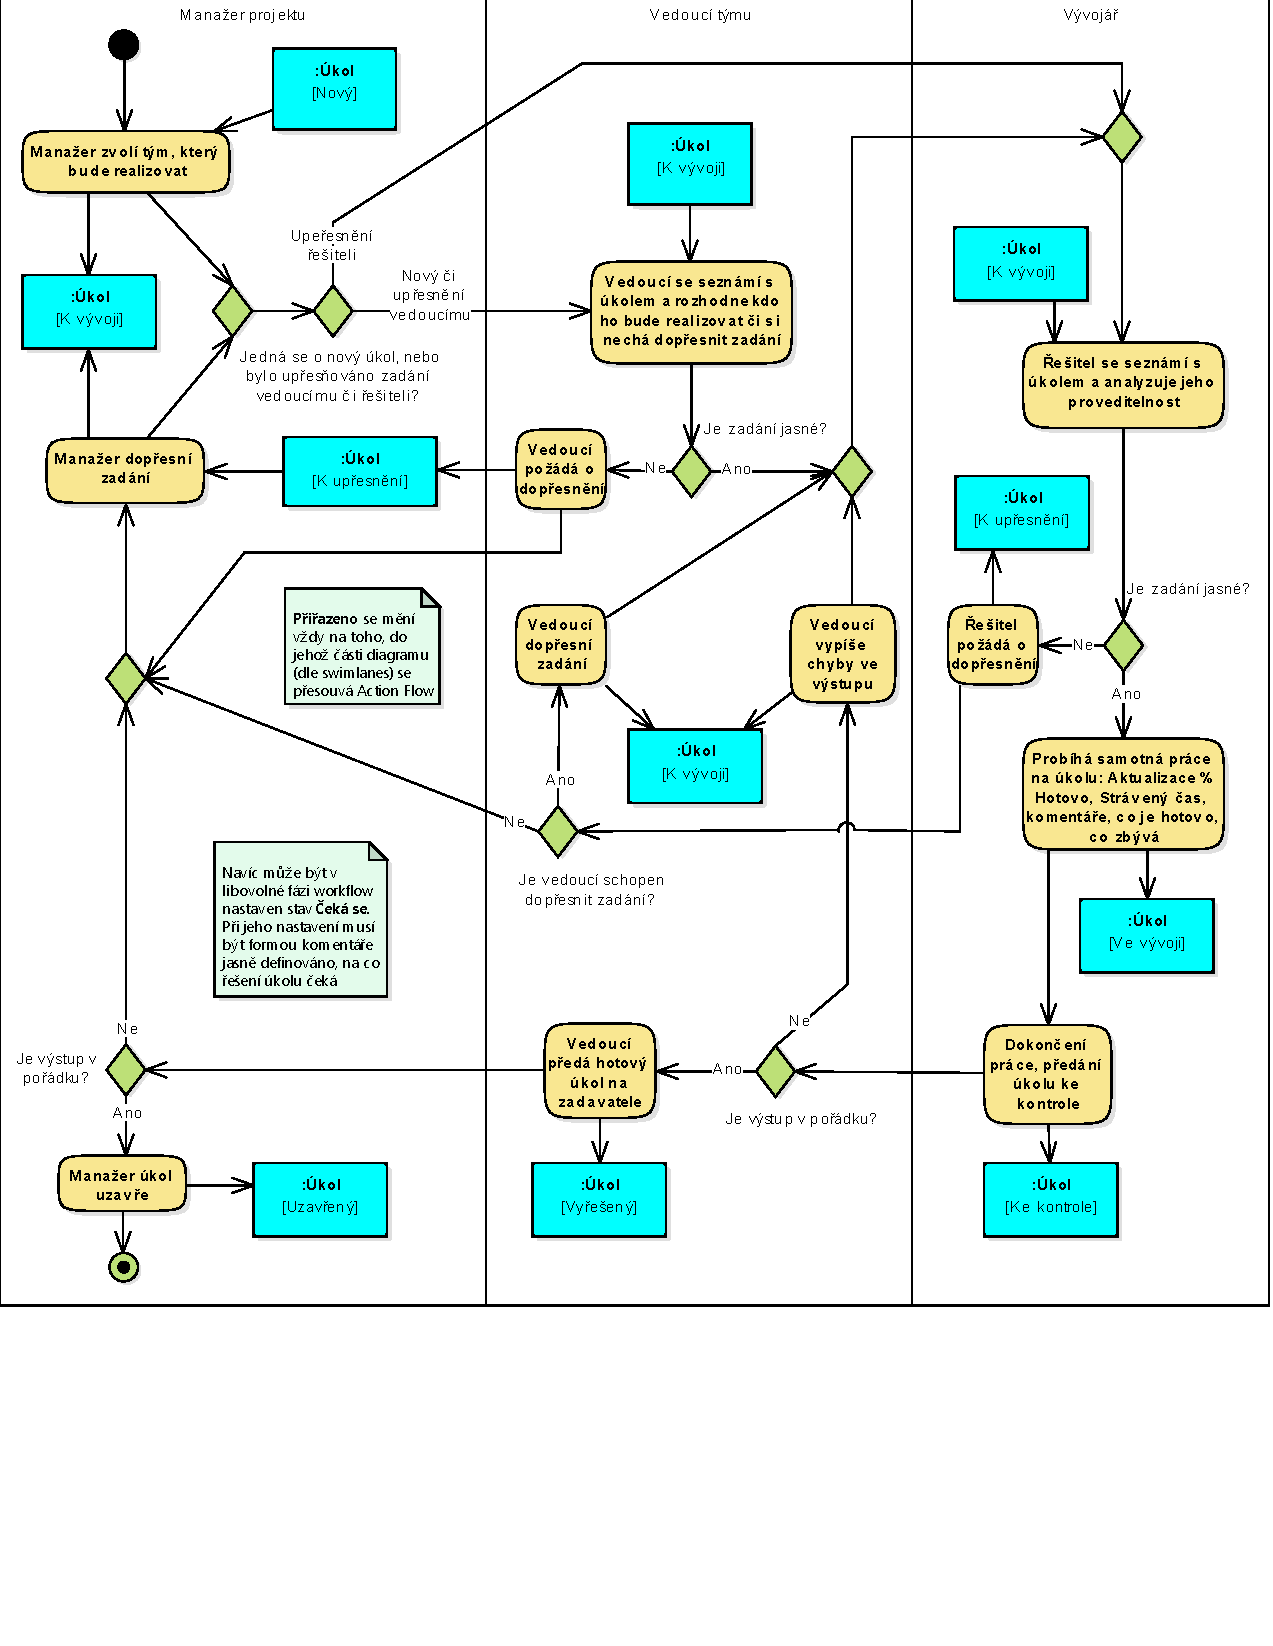
\includegraphics[width=\textwidth]{../pdf/dbs-workflow.pdf}
\caption{Activity diagram průběhu práce v Redmine} \label{picture:activity}
\end{figure}

\chapter{Vstupní kvíz} \label{ap:quiz}

\begin{figure}[h]
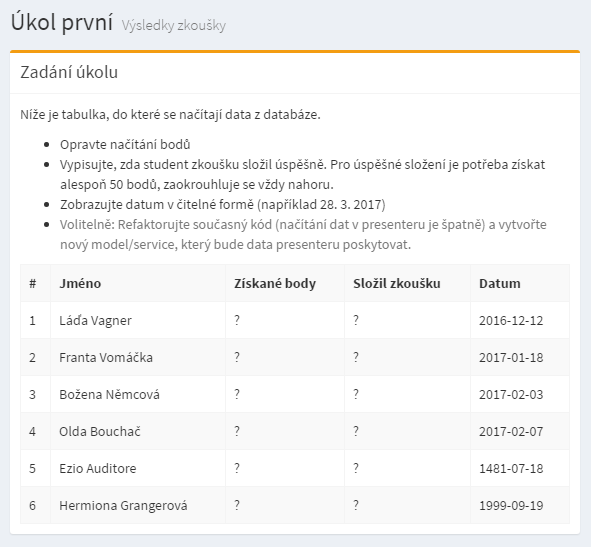
\includegraphics[width=\textwidth]{../png/quiz-1.png}
\caption{První úloha vstupního kvízu DBS projektu. Autor: Oldřich Malec} \label{picture:quiz-1}
\end{figure}

\begin{figure}[]
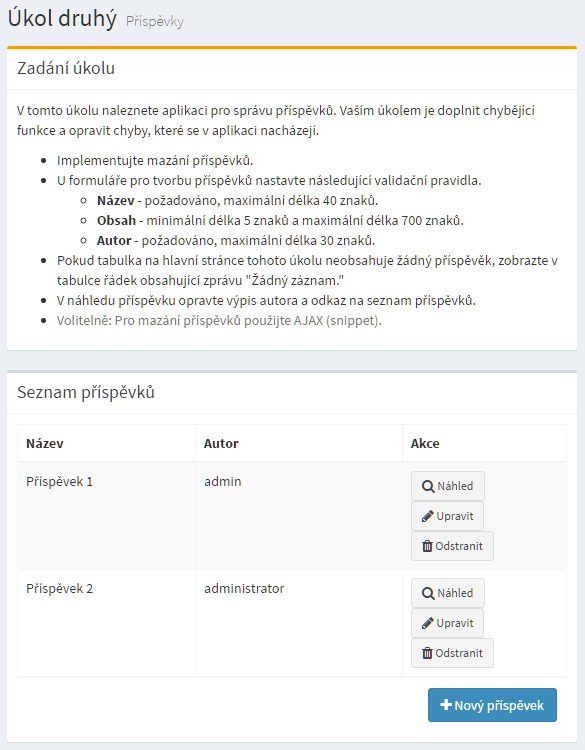
\includegraphics[width=\textwidth]{../png/quiz-2.png}
\caption{Druhá úloha vstupního kvízu DBS projektu. Autor: Pavel Kovář} \label{picture:quiz-2}
\end{figure}

\begin{figure}[]
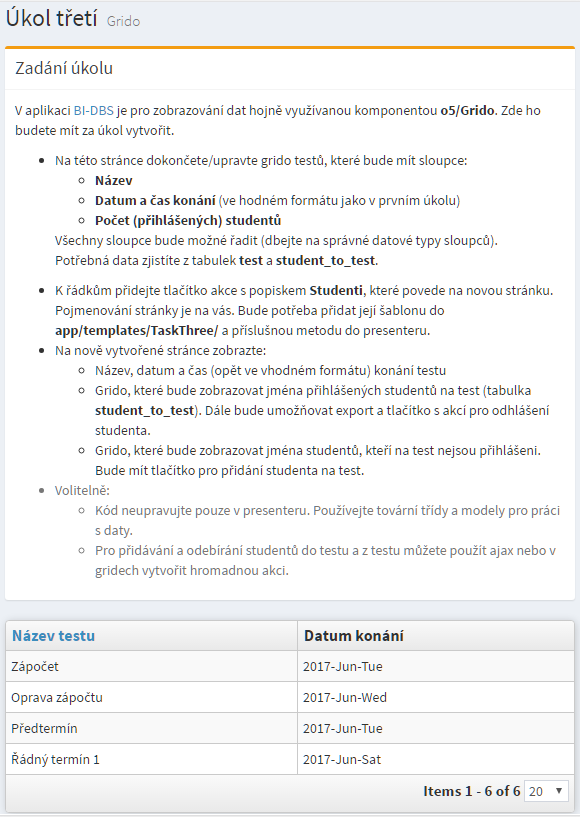
\includegraphics[width=\textwidth]{../png/quiz-3.png}
\caption{Třetí úloha vstupního kvízu DBS projektu. Autor: Milan Vlasák} \label{picture:quiz-3}
\end{figure}

\chapter{Hodnocení týmů} \label{ap:ranking}

\begin{sidewaysfigure}[]
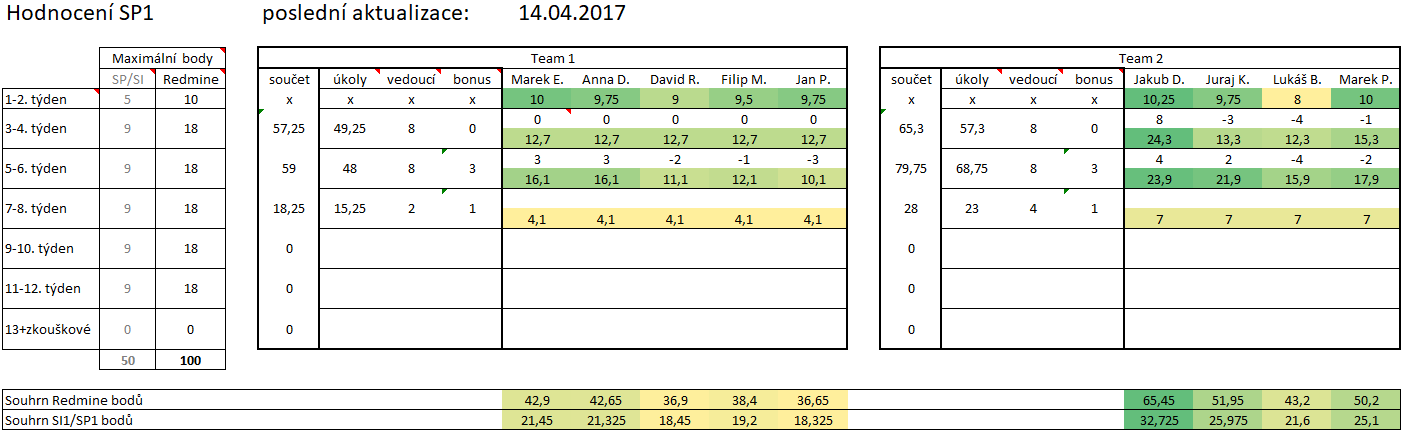
\includegraphics[width=\textwidth]{../png/ranking.png}
\caption{Tabulka hodnocení týmů} \label{picture:ranking}
\end{sidewaysfigure}


\end{document}